\sectionquestion{TA QUESTIONS GO HERE!!!}

\subsection{Decision Trees}
\begin{parts}

\part We have seen classification with decision trees in the lectures. In this question, we will perform regression with decision trees. Let us assume that we have N data samples to train on with their non discrete target values. We have a separate set of M samples for testing. 
\begin{subparts}
    \subpart[1] \textbf{Short answer} Let us say you have already built a tree with the data above. In decision trees, each leaf node corresponds to a fixed prediction value. What would be this fixed prediction value at the leaves which provides us with the least mean squared error at the leaves for the regression decision tree?
    \fillwithlines{2em}
    \begin{soln}
    Mean of the samples associated to the leaf.
    \end{soln}
    \begin{qauthor}
        Varsha, Design k-NN Regression and Decision Tree Regression
    \end{qauthor}
    \begin{qtester}
   I think this is a little unclear. Couldn't you use median? Or a function of the data points? Would we accept all answers?
    \end{qtester}
    
    
    \subpart[3] \textbf{Short answer} How do you build the tree from the N samples provided? Clearly mention the splitting criterion and the cost function. You don't have to worry about overfitting in this part.
    \fillwithlines{2em}
    \begin{soln}
    We can split the data along individual features.
    The cost function is the MSE equation.
    Splitting criterion: Split the data at the level of a single feature such that splitting it reduces the final MSE.
    \end{soln}
    \begin{qauthor}
        Varsha, Design k-NN Regression and Decision Tree Regression
    \end{qauthor}
    \begin{qtester}
   Again I think we could get multiple answers here. Which learning objective is this addressing? It seems out of scope.
    \end{qtester}
    
    
    \subpart[2] \textbf{Short answer} How do you tackle overfitting in regression decision trees?
    \fillwithlines{2em}
    \begin{soln}
    First split the data into train and validation sets. We can first build a complete tree from the train samples and then prune the tree. Pruning can be done greedily considering the merge which gives us best performance on the validation data.
    \end{soln}
    \begin{qauthor}
        Varsha, Design k-NN Regression and Decision Tree Regression
    \end{qauthor}
    \begin{qtester}
   I think regression DTs are out of scope for this exam, but this part of the question could be adapted for classification
    \end{qtester}
\end{subparts}
\end{parts}

\subsection{kNNs}
\begin{parts}
    \part \textbf{Short Answer:} Suppose we create the following variant of the k-NN Algorithm with k=4 and euclidean distance metric for a binary classification task (+1 or -1): $\hat{y}^{(i)} = sign(2y_1 + y_2 + y_3 + y_4)$, where $y_i$ is the class of the i-th closest point to y ($i = 1, 2, \cdots, 4$). Essentially, we are giving double the weight to the closest point. If there is a tie for the closest point to y, then we choose an arbitrary point to get double the vote. Your friend claims that ties in the vote will never happen(i.e the value inside the sign expression will never be 0). Is your friend correct? \\ \\
    
    \begin{tcolorbox}[fit,height=4cm, width=15cm, blank, borderline={1pt}{-2pt}, nobeforeafter=false]
    \end{tcolorbox}
    \fillwithlines{2em}
    \begin{soln}
    Your friend is correct. Since each point is classified as +1 or -1, with three points, the only possible values for the sum is +1 or -1. The value for the closest point is either +2 or -2, which means that if we add the values of all the points with the weights, we will never get 0.
    \end{soln}
    \begin{qauthor}
    Bhargav, Invent "new" k-NN learning algorithms capable of dealing with even k
    \end{qauthor}

    \part You are given a training dataset containing information about various species of strawberries. Each species is described by its sweetness (on a scale from 0 to 5), and weight (in grams). You want to use $k$-NN to classify which species are popular. You create a binary label (+/-) based on the popularity such that you assign a label of + if the species is popular and - otherwise. Consider the following data set:
\begin{align*}
    D &= \{(x^{(i)}, y^{(i)}\}_{i=1}^{7}\\
    &= \{((1,3),+),((2,1),-),((2,5), +), ((3,2), -),((3,3),-),((4,1),+),((4,4),+)\}
\end{align*}
where $x^{(i)} \in \mathbf{R}^{2} = (\text{weight}, \text{sweetness})$ and $y^{(i)} \in \{+, -\}$ is the label.

Next, you train your k-NN model on this training data set. The distance measure you use is Euclidean distance. Assume the ties are broken by selecting less sweet and less heavy species. (Example tie scenario: if $k=2$, $(1,3)$ and $(3,3)$ have the same euclidean distance with $(2,3)$, then we choose $(1,3)$ as the closest point.)

\begin{subparts}
    \subpart[2] \textbf{Drawing:} Given the training dataset shown above, plot each data point in the graph below by using + or -:

    \begin{center}
        \begin{tikzpicture}
        \begin{axis}[
            scale=1.5, axis equal image, mark options={scale=1.5},
            xmin=0, xmax=6, xtick={1,...,5},
            ymin=0, ymax=6, ytick={1,...,5},
            samples=50, grid=major, xlabel= Weight, ylabel=Sweetness]]
        \end{axis}
        \end{tikzpicture} 
    \end{center}
    \begin{soln}
    \begin{center}
    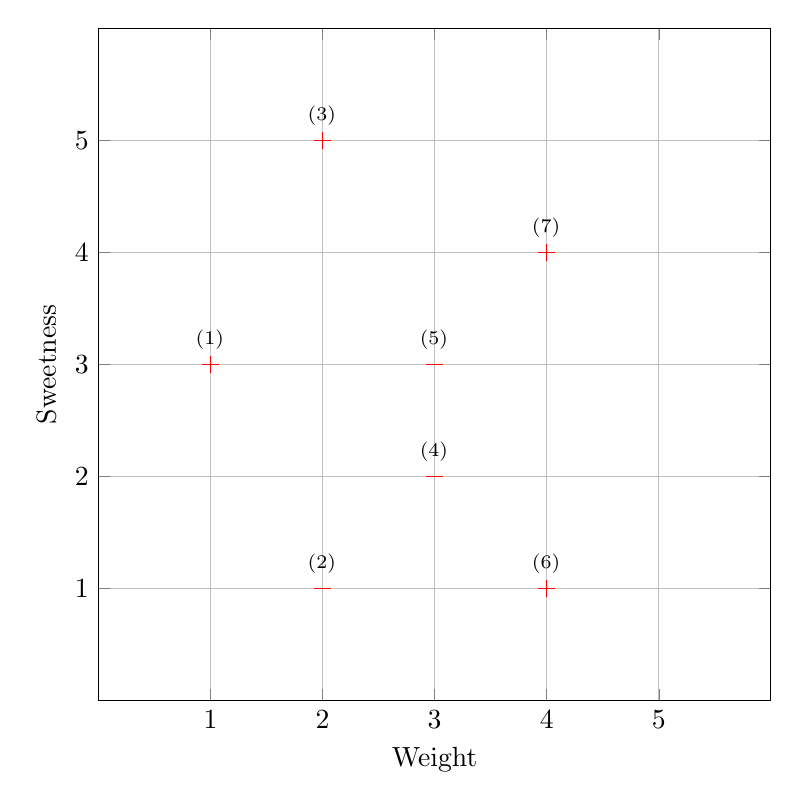
\begin{tikzpicture}
    \begin{axis}[
        scale=1.5, axis equal image, mark options={scale=1.5},
        xmin=0, xmax=6, xtick={1,...,5},
        ymin=0, ymax=6, ytick={1,...,5},
        samples=50, grid=major, xlabel=Weight, ylabel=Sweetness]]
        \addplot [
            scatter,
            only marks,
            point meta=explicit symbolic,
            scatter/classes={
                a={mark= +,red},
                b={mark= -,red}
            },
            nodes near coords*={$\xv^{(\pgfmathprintnumber[frac]\myvalue)}$},
            visualization depends on={\thisrow{myvalue} \as \myvalue},
        ] table [meta=label] {
            x y label myvalue
            1 3 a 1
            2 1 b 2
            2 5 a 3
            3 2 b 4
            3 3 b 5
            4 1 a 6
            4 4 a 7
        };
    \end{axis}
    \end{tikzpicture}   
\end{center}
    \end{soln}
    \begin{qauthor}
    Zoe Xu, Describe a dataset as points in a high dimensional space
    \end{qauthor}

    \subpart[5] \textbf{Drawing:} Given the training dataset shown above, draw the decision boundary for $k=1$.
    
    
    \subpart[2] \textbf{Numerical answer:} Choosing $k = 3$, what is the training error? \textbf{Report your answer as a fraction.}
    \begin{tcolorbox}[fit,height=1cm, width=2cm, blank, borderline={1pt}{-2pt}]
    %solution
    \end{tcolorbox}
    \begin{soln}
    $\frac{3}{7}$
    \end{soln}
    \begin{qauthor}
        Zoe Xu, implement $k$-NN algorithm and deal with tie scenario.
    \end{qauthor}

\begin{qtester}
    Should this be 3/7? x1, x7, x6?
    
    Zoe: Yes! Thank you very much. I should look at the answer more carefully.
\end{qtester}
    
    \subpart[4] \textbf{Select all that apply:} Let's say we have a new species with weight 2 and sweetness 3, and the new species is \textbf{not} popular among the market. For which values of $k$ is this new species always correctly classified by the $k$-NN algorithm?
\checkboxchar{$\Box$} \checkedchar{$\blacksquare$} % change checkbox style locally
    \begin{checkboxes}
     \choice $k = 1$
     \choice $k = 2$
     \choice $k = 3$
     \choice $k = 4$
     \choice None of the above
    \end{checkboxes}
    \begin{soln}
    $B, D$
    \end{soln}
    \begin{qauthor}
        Zoe Xu, implement $k$-NN algorithm and deal with tie scenario.
    \end{qauthor}
    \begin{qtester}
    At this point we are testing, so k=1 should not be valid right? 

    Zoe Xu: Yes! You're right. Thanks again!s
    \end{qtester}

    \subpart[2] \textbf{Short answer:} Looking at the training errors, you choose the model with $k = 1$ as it has the lowest training error. Do you think this is the right approach to select a model? Why or why not?

    \begin{soln}
    No, we would use validation dataset (validation error) to choose k as k is a hyperparameter.
    \end{soln}
    \begin{qauthor}
        Zoe Xu (citing from practice problem Exam1 F23), one point for true or false, and one point for reason.
        Describe the inductive bias of a $k$-NN classifier
    \end{qauthor}

    \subpart[3] \textbf{Select all that apply:} Please select all that apply about $k$-NN in the following options. Assume a point can be its own neighbor.
    \checkboxchar{$\Box$} \checkedchar{$\blacksquare$} % change checkbox style locally
    \begin{checkboxes}
     \choice $k$-NN can be applied to classification problems but not regression problems.
     \choice We can always achieve zero training error with $k$-NN, but it may not generalize well in testing.
     \choice We usually decrease $k$ to avoid over-fitting.
     \choice $k$-NN is computationally slow when the number of features is large.
     \choice None of the above
    \end{checkboxes}
    \begin{soln}
    $B, D$
    \end{soln}
    \begin{qauthor}
        Zoe Xu, test understanding of $k$-NN model
    \end{qauthor}
\end{subparts}
\end{parts}

\subsection{Perceptron}
\begin{parts}
\part[2] \textbf{Short answer:} You will be asked to modify the perceptron algorithm in this question. Here is the algorithm as discussed in the class.

    \fbox{\parbox{\textwidth}
    {\begin{itemize}
        \item Initialize the weight vector and intercept to all zeros:
        $$
        \boldsymbol{w}=\left[\begin{array}{llll}
        0 & 0 & \cdots & 0
        \end{array}\right] \text { and } b=0
        $$
        \item For $t=1,2,3, \ldots$
            \begin{itemize}
                \item Receive an unlabeled data point, $\boldsymbol{x}^{(t)}$
                \item Predict its label:
                \[
                \hat{y} = \text{sign}\left(\boldsymbol{w}^T \boldsymbol{x}^{(t)} + b\right) =
                \begin{cases}
                    +1 & \text{if } \boldsymbol{w}^T \boldsymbol{x}^{(t)} + b \geq 0 \\
                    -1 & \text{otherwise}
                \end{cases}
                \]
                \item Observe its true label, $y^{(t)}$
                \item If misclassified ($y^{(t)} \neq \hat{y}$):
                \[
                \begin{aligned}
                    & \cdot \boldsymbol{w} \leftarrow \boldsymbol{w} + y^{(t)} \boldsymbol{x}^{(t)} \\
                    & \cdot b \leftarrow b + y^{(t)}
                \end{aligned}
                \]
            \end{itemize}
    \end{itemize}}}

    % \begin{subparts}
    % \subpart[2] 
    Modify the standard perceptron algorithm such that it produces the classifier with maximum margin between classes. As a reference, here is an image depicting two classifiers which a perceptron can return on a linearly separable data. You goal is to modify the algorithm such that it always tends to return $h_{1}$.
    \begin{figure}[htbp]
      \centering
      \includegraphics[width=0.5\textwidth]{figures/perceptron_margin}
    \end{figure}
    \fillwithlines{2em}
    \begin{soln}
    Here is a brief algorithm:
    \begin{itemize}
        \item We would first normalize the input samples. Initialize $\mathbf{w}_1=\mathbf{y} \mathbf{x}$, where $\mathbf{x}$ is the first example seen and initialize $t$ to 1.
        \item Predict positive if $\frac{\mathbf{w}_t \cdot \mathbf{x}}{\left\|\mathbf{w}_t\right\|} \geq \gamma / 2$, predict negative if $\frac{\mathbf{w}_t \cdot \mathbf{x}}{\left\|\mathbf{w}_t\right\|} \leq-\gamma / 2$, and consider an example to be a margin mistake when $\frac{\mathbf{w}_t \cdot x}{\left\|\mathbf{w}_t\right\|} \in(-\gamma / 2, \gamma / 2)$.
        \item On a mistake (incorrect prediction or margin mistake), update as in the standard Perceptron algorithm: $\mathbf{w}_{t+1} \leftarrow \mathbf{w}_t+\mathbf{y} \mathbf{x} ; t \leftarrow t+1$.
    \end{itemize}
    \end{soln}   
    \begin{qauthor}
    Varsha, If the students come up with the second and third parts to some extent, we can give them complete credit.
    \end{qauthor}

    \begin{qtester}
   This may be a little difficult. We do not talk about margins much until SVMs. I don't think this was covered with Perceptron. Which learning objective is this addressing?
    \end{qtester}

    \part In this question you will have to answer some questions regarding the perceptron algorithm.
    \begin{subparts}
    \subpart[1] \textbf{Short Answer: }Consider a supervised learning problem with N examples, each of which is a point in d-dimensional space. Let us say our perceptron has converged after t iterations. What is the runtime complexity of the algorithm as a function of N, d, and t? Give a brief explanation of your answer.
    \fillwithlines{1em}
    \begin{soln}
         O(N * d * t), t iterations, each iteration we would perform a dot product which takes O(d) for N samples.
    \end{soln}
    \begin{qauthor}
    Varsha, Implement the perceptron algorithm for binary classification
    \end{qauthor}

    \subpart[2]\textbf{Short Answer: }Let us say we have a learning problem where each input is of d dimensions. Each of these d feature values can only take values 0 or 1. Design a perceptron which classifies the samples as positive if the number of 1s in the feature values of the input is more than the number of 0s. 
    
    \fillwithlines{1em}
    \begin{soln}
         We can have a perceptron where all the weights for d features is 1, and bias term is ceil(-(d+1)/2). (We can get this solution algebraically)
    \end{soln}
    \begin{qauthor}
    Varsha
    \end{qauthor}
    \end{subparts}
\end{parts}

\subsection{Linear Regression}
\begin{parts}

\part[2] \textbf{Numerical answer:} For a linear regression model assume the learning rate $\alpha$ is $0.1$ and the initial value of parameters $\theta_0$ is $0$ and $\theta_1$ is $1$. The training set has 3 samples with the following values:
\begin{center}
    \begin{tabular}{c|c}
		\hline
		x_1& y\\
	    \hline
		1&3 \\
  		3&5 \\
            4&8 \\
		\hline
    \end{tabular}
\end{center}

Use the gradient descent update rule to find the value of parameter $\theta_1$ after one iteration. 
    \begin{tcolorbox}[fit,height=1cm, width=2cm, blank, borderline={1pt}{-2pt}]
    %solution
    \end{tcolorbox}
    \begin{soln}
    1.8
    \end{soln}
    \begin{qauthor}
    Kushagra Agarwal, Implement learning for Linear Regression using ONE optimization technique:(2) gradient descent (the others are saved for Exam 2).
    \end{qauthor}

\part[2] \textbf{Numerical answer:} Suppose you have a quadratic function  $f(x) = 6x^2 - 3x + 5$ that you want to minimize using gradient descent. Apply the gradient descent algorithm with a learning rate $\alpha$ of $0.1$, starting from an initial guess $x=2$ and calculate the new value of $x$ after one iteration.
    \begin{tcolorbox}[fit,height=1cm, width=2cm, blank, borderline={1pt}{-2pt}]
    %solution
    \end{tcolorbox}
    \begin{soln}
    $-0.1$
    \end{soln}
    \begin{qauthor}
    Kushagra Agarwal, Apply gradient descent to optimize a function
    \end{qauthor}
    
\part Suppose that we are an adversary that wants to do \textit{as poorly as possible} on some decision task. This logic has applications to fields such as robust and fair ML, where developers must consider the worst-case performance of their model over a set of plausible distributions of individuals. However, rather than investigating worst-case performance over distributions, we consider worst-case performance on a fixed set $X, Y$, over \textbf{model parameters} $\theta$. 

\begin{subparts}
    
    \subpart[2] \textbf{Short answer}: Write the objective function for this new problem setup, using the variables $\theta \in \mathbb{R}^{M}$ to denote the parameter of interest, $\hat{\theta}$ for the estimated solution of interest, and $J$ to represent the (arbitrary) objective function.

    \begin{soln}
    \begin{align*}
        \hat{\theta} = \argmax_{\theta \in \mathbb{R}^M} J(\theta)
    \end{align*}
    \end{soln}
    
    \subpart[2] \textbf{Short answer}: Explain why the use of this objective for linear regression is flawed in an unconstrained optimization setting.
    
    \begin{soln}
        Note that in this setting, we can make $\hat{\theta}$ \textbf{arbitrarily bad} leading to degenerate solutions if no constraints are imposed on its values. For example, you could adversarially set the values within $\theta$ to approach $\pm \inf$, and as you keep shifting $\theta$ to arbitrarily large-magnitude values, your predictions would become arbitrarily farther away from the solutions, meaning finding an argmax could entail $\theta_i = \pm \inf, 0 \leq i \leq M$.
    \end{soln}

    \subpart[2] \textbf{Short answer}: Propose one way we could ameliorate the above problem.

    \begin{soln}
        Imposing constraints on $\hat{\theta}$, e.g. $||\hat{\theta}||_2^2 \leq \epsilon, \epsilon \in \mathbb{R}$, or $|\hat{\theta} - \theta^*| \leq \epsilon$, where $\theta^*$ denotes the value of $\theta$ that minimizes the objective functions (e.g. OLS solution for 'regular' linear regression; we say that the worst-case $\hat{\theta}$ cannot stray too far from a 'good' solution to the optimization problem)
    \end{soln}
\end{subparts}

\begin{qauthor}
    (1) Kevin, (2) objective functions/closed form solutions in OLS
\end{qauthor}

\part[2] \textbf{Short answer}:
    Consider the following loss function $\ell$, which uses the \textit{absolute value} of the residual between a label $Y$ and its estimation $\hat{Y} = \theta X + \theta_0$, where $X$ is a feature vector and $\theta, \theta_0$ represent a learned set of parameters for regression:
    \begin{align*}
        \ell(Y, \hat{Y}) = |Y - \hat{Y}|
    \end{align*}
    We would like to use $\ell$ in place of residual sum of squares (RSS) when identifying loss over a matrix of training data $X$ and labels $Y$ containing $n$ individuals each, e.g.

    \begin{align*}
        L(X, Y) = \frac{1}{n} \sum_{i = 1}^{n} \ell(Y_i, \theta(X_i) + \theta_0)
    \end{align*}
    
    If possible, provide the closed-form solution to an adaptation of linear regression using the sum of absolute values of residuals $\ell$ in place of RSS. If this is not possible, provide a brief justification as to why, and a potential alternative solution.
    
\begin{soln}
    This is not possible, because the loss function is not differentiable w.r.t. $\hat{y}$ and therefore $x$. As a result, the MLE methods that make a closed-form solution for OLS possible are not applicable to $\ell$. Linear programming/algorithmic approaches on the data should still be able to yield an approximate solution, however.
\end{soln}

\begin{qauthor}
    (1) Kevin, (2) importance of differentiable loss functions in developing closed-form sollutions; consideration of algorithmic techniques for optimization
\end{qauthor}

\part[2] \textbf{Select one}: Consider the following methods of determining whether gradient descent for (unconstrained) OLS linear regression has converged yet. Which of the following would not be valid ways of doing so?

\begin{checkboxes}
    \choice stopping once the L2 norm of the gradient w.r.t. the estimated solution $\theta$ is less than some constant $\epsilon$
    \choice stopping after a fixed set of iterations of gradient descent
    \choice stopping once the L2 norm of the solution $\theta$ is less than a threshold $\epsilon$
    \choice stopping once the change in the objective function from one iteration $t$ to the next iteration $t+1$ is less than a threshold $\epsilon$, e.g. $J(\theta_t; X,Y) - J(\theta_{t+1}; X,Y) \leq \epsilon$
\end{checkboxes}

\begin{soln}
    C
\end{soln}

\begin{qauthor}
    (1) Kevin, (2) stopping conditions in gradient descent for OLS
\end{qauthor}

\begin{qauthor}
    (1) Kevin, (2) importance of differentiable loss functions in developing closed-form sollutions; consideration of algorithmic techniques for optimization
\end{qauthor}
\end{parts}

\subsection{Other/Miscellaneous/Multiple Topics}
\begin{parts}


\part[2] \textbf{Select one:} When we train machine learning models, why do we try to minimize the training error instead of directly minimizing the true error?
    \begin{checkboxes}
     \choice It is possible to calculate the true error, but it is very computationally expensive to find it, so we use the training error instead.
     \choice We don't. With a reasonably large dataset, training error and true error are exactly the same thing.
     \choice Determining the true error requires you to have access to a training dataset that contains every single possible input and output to the model.
     \choice Using the training error instead of the true error guarantees that your learning algorithm will converge.
    \end{checkboxes}
    \begin{soln}
    C. You cannot calculate the true error, since you need to have access to every single point in the domain to do so (and also an accurate error metric). 
    \end{soln}
    \begin{qauthor}
    Rohan Chawla, Explain the difference between true error and training error.
    \end{qauthor}

\end{parts}




